\section{評価}
\label{section:評価}
\subsection{Service Workerのパフォーマンス}
\label{subsection:Service Workerのパフォーマンス}
Lighthouseとネットワークスロットリングを使用して、それぞれの都道府県の観光地図を読み込んだ際のパフォーマンスを計測した。キャッシュ戦略ごとのパフォーマンス指標の値の平均を図~\ref{figure:Service Workerを使用しなかった場合のパフォーマンス}、~\ref{figure:画像をキャッシュした場合のパフォーマンス}、~\ref{figure:Same-Originのネットワークレスポンスをキャッシュした場合のパフォーマンス}、表~\ref{table:全てのネットワークレスポンスをキャッシュした場合のパフォーマンス}に示す。
\begin{figure}
  \centering
  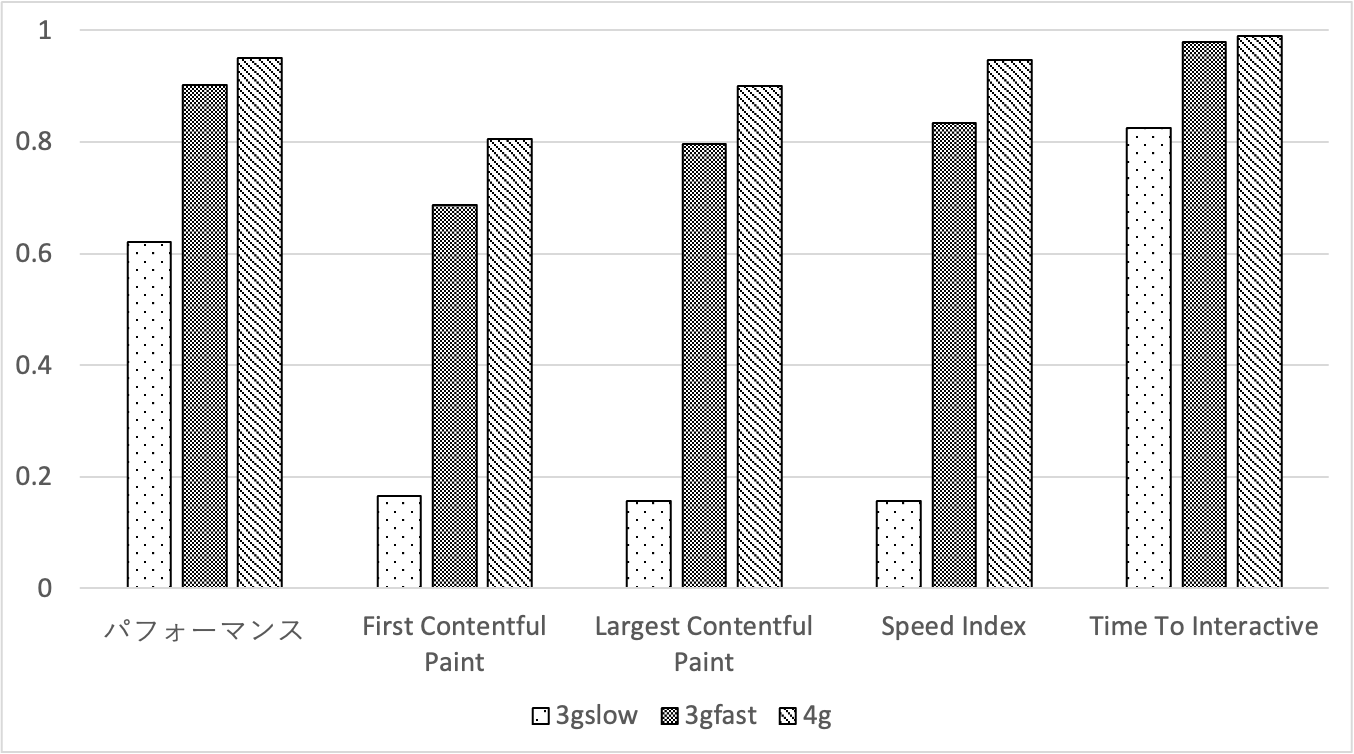
\includegraphics[width=\textwidth]{images/without_service_worker.png}
  \caption{Service Workerを使用しなかった場合のパフォーマンス}\label{figure:Service Workerを使用しなかった場合のパフォーマンス}
\end{figure}
\begin{table}
  \caption{全てのネットワークレスポンスをキャッシュした場合のパフォーマンス}
  \label{table:全てのネットワークレスポンスをキャッシュした場合のパフォーマンス}
  \centering
  \begin{tabular}{|p{15em}|p{5em}|p{5em}|p{5em}|}
    \hline
    & 3gslow & 3gfast & 4g \\ \hline
    パフォーマンス & 1 & 1 & 1 \\ \hline
    First Contentful Paint & 1 & 1 & 1 \\ \hline
    Largest Contentful Paint & 1 & 1 & 1 \\ \hline
    Speed Index & 1 & 1 & 1 \\ \hline
    Time To Interactive & 1 & 1 & 1 \\ \hline
    Total Blocking Time & 1 & 1 & 1 \\ \hline
    Cumulative Layout Shift & 1 & 1 & 1 \\ \hline
  \end{tabular}
\end{table}
\begin{figure}
  \centering
  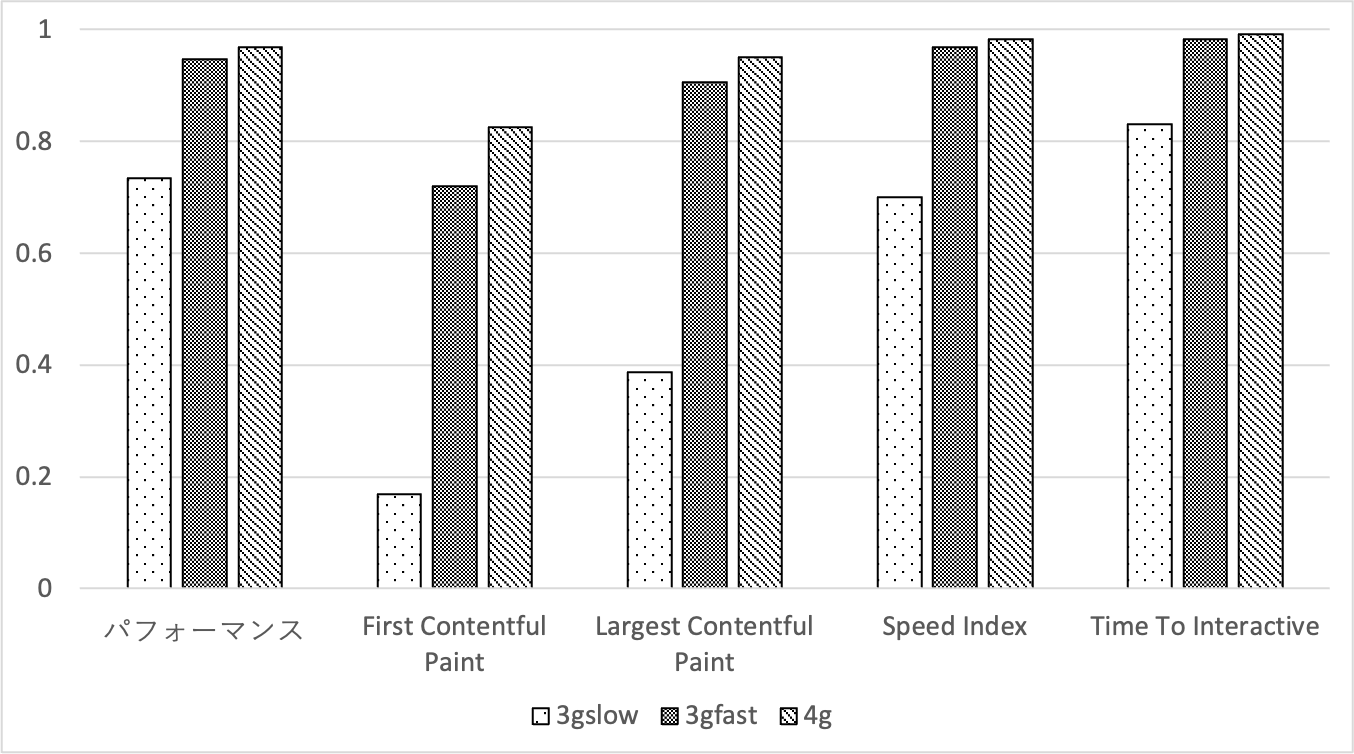
\includegraphics[width=\textwidth]{images/service_worker_cache_images.png}
  \caption{画像をキャッシュした場合のパフォーマンス}\label{figure:画像をキャッシュした場合のパフォーマンス}
\end{figure}
\begin{figure}
  \centering
  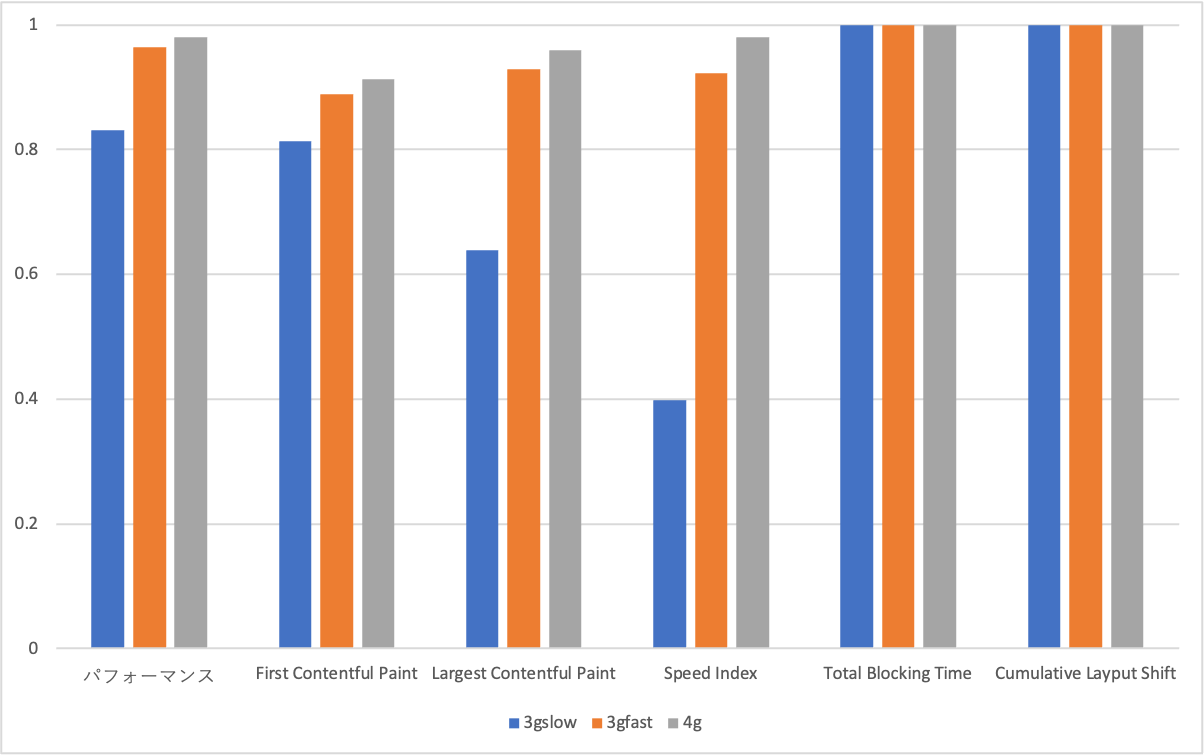
\includegraphics[width=\textwidth]{images/service_worker_cache_same_origin.png}
  \caption{Same-Originのネットワークレスポンスをキャッシュした場合のパフォーマンス}\label{figure:Same-Originのネットワークレスポンスをキャッシュした場合のパフォーマンス}
\end{figure}
いずれの場合もTBTとCLSは1である。4g、3gfast、3gslowの順でパフォーマンス指標の値が大きい傾向にある。全てのネットワークレスポンスをキャッシュした場合は3gslow、3gfast、4gのいずれの場合も全ての指標の値は1である。画像をキャッシュした場合はFCPが最も通信速度の低下の影響を受けやすく、SIが最もその影響を受けにくいことが分かる。逆に、Same-Originのネットワークレスポンスのキャッシュした場合はSIが最も通信速度の低下の影響を受けやすく、SCPが最もその影響を受けにくいことが示されている。

3gfastに比べてアップリンクがおよそ12倍、ダウンリンクがおよそ6倍である4gプロファイルを使用した場合であってもほとんどのパフォーマンス指標の値は1未満である。全体的に見ると、3gslowと3gfast間のパフォーマンス指標の値の増加率は3gfastと4g間の増加率よりも大きい。

Same-Originのネットワークレスポンスをキャッシュした場合はいずれのネットワーク環境においてもTTIがほぼ1である。対照的に、画像をキャッシュした場合のTTIはService Workerを使用しなかった場合のTTIとほとんど同じであるため、画像のキャッシュはTTIにほとんど影響を及ぼさないことが分かる。

\subsection{ユーザーの操作に基づいて読み込まれたリソースの処理時間}
\label{subsection:ユーザーの操作に基づいて読み込まれたリソースの処理時間}
読み込みのみ、読み込みとスクロール、読み込みとズームの操作時に読み込まれた1都道府県当たりの画像の枚数を図~\ref{figure:操作時に読み込まれた1都道府県当たりの画像の枚数}に示す。

\begin{figure}
  \centering
  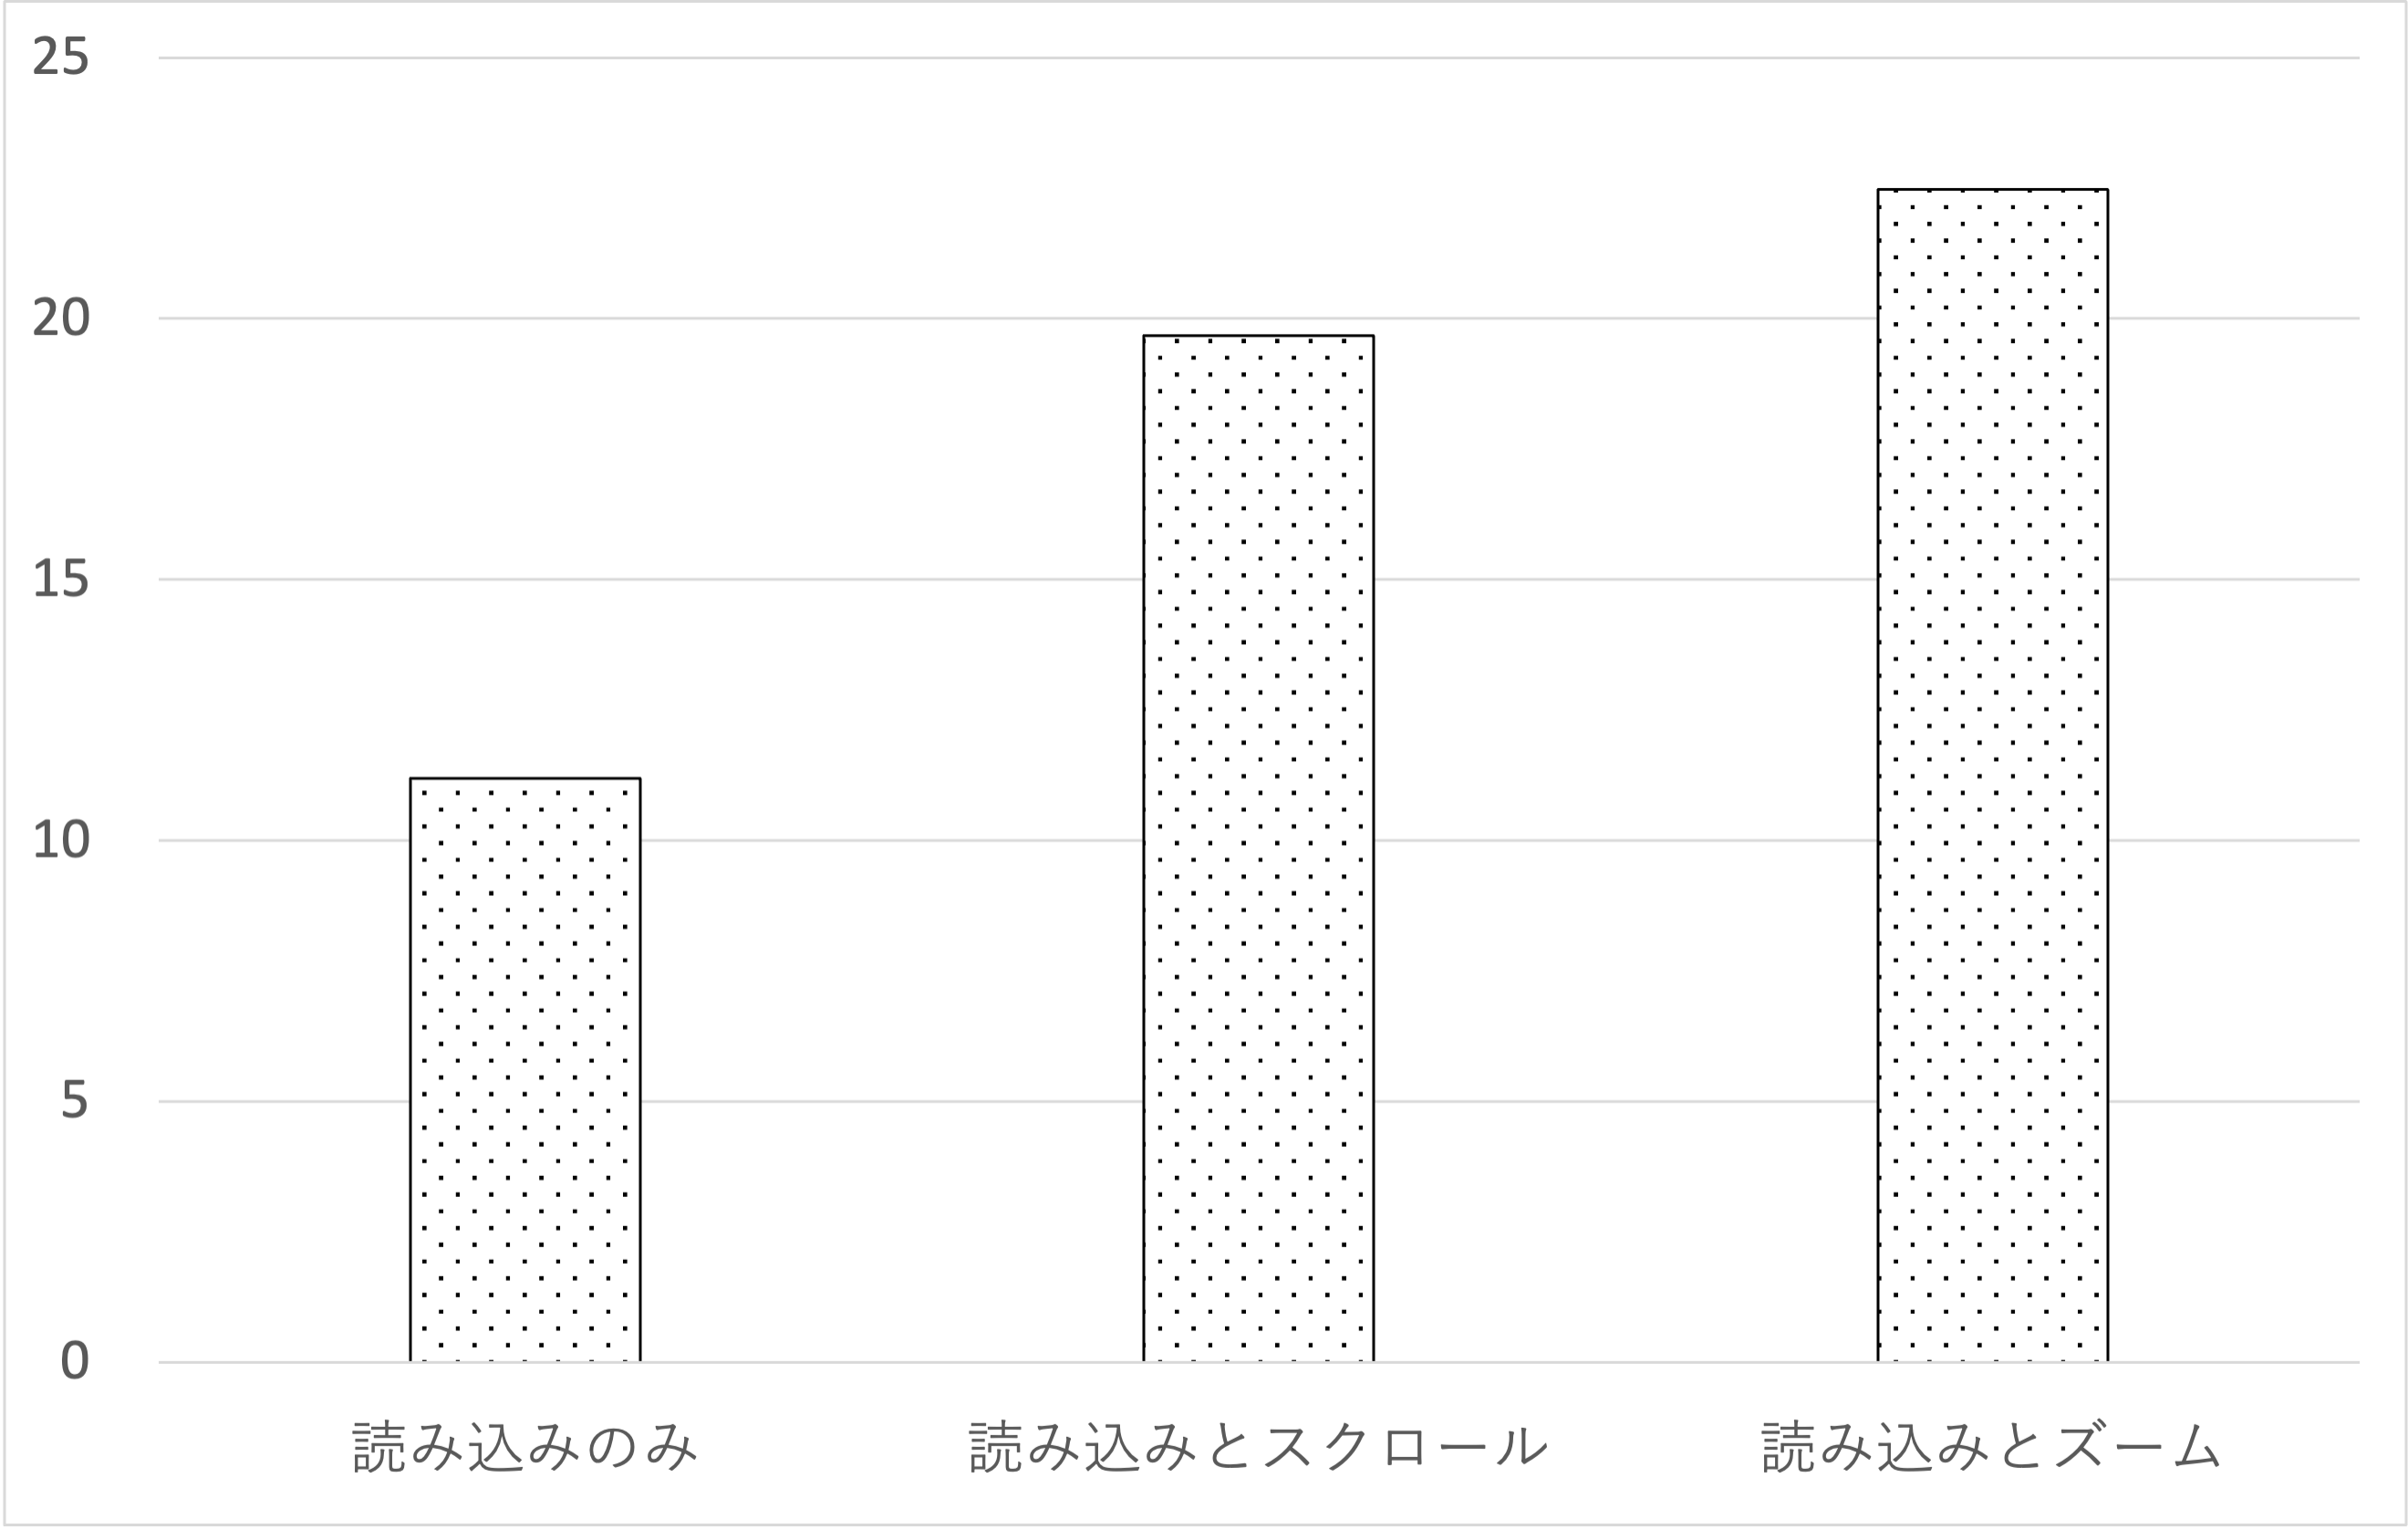
\includegraphics[width=\textwidth]{paper/images/loaded_image_count.png}
  \caption{操作時に読み込まれた1都道府県当たりの画像の枚数}\label{figure:操作時に読み込まれた1都道府県当たりの画像の枚数}
\end{figure}

1ページ下にスクロールした場合はスクロール前とスクロール後の両方で使用されている画像があるため、読み込まれる画像の枚数が2倍未満であることに注意が必要である。その一方で、ズーム倍率を1だけ増加させた場合は、読み込みのみの場合と比べて2倍の枚数の画像が読み込まれることが分かる。

次に、Service Workerを使用しない場合の、1都道府県当たりの画像の読み込み時間の合計平均を図~\ref{figure:Service Workerを使用しない場合の1都道府県当たりの画像の読み込み時間の合計平均}に、Service Workerを使用する場合の1都道府県当たりの画像の読み込み時間の合計平均を図~\ref{figure:Service Workerを使用する場合の1都道府県当たりの画像の読み込み時間の合計平均}に示す。

\begin{figure}
  \centering
  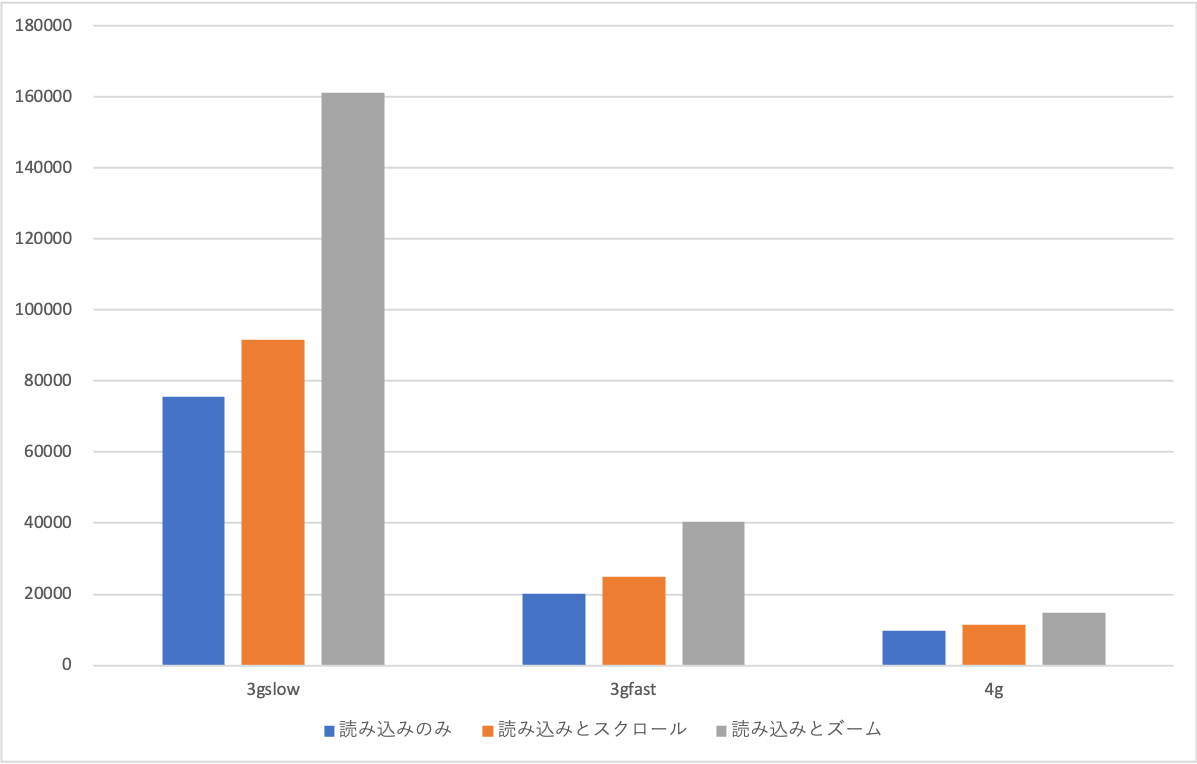
\includegraphics[width=\textwidth]{paper/images/sum_of_image_durations_without_service_worker.png}
  \caption{Service Workerを使用しない場合の1都道府県当たりの画像の読み込み時間の合計平均[ミリ秒]}\label{figure:Service Workerを使用しない場合の1都道府県当たりの画像の読み込み時間の合計平均}
\end{figure}

\begin{figure}
  \centering
  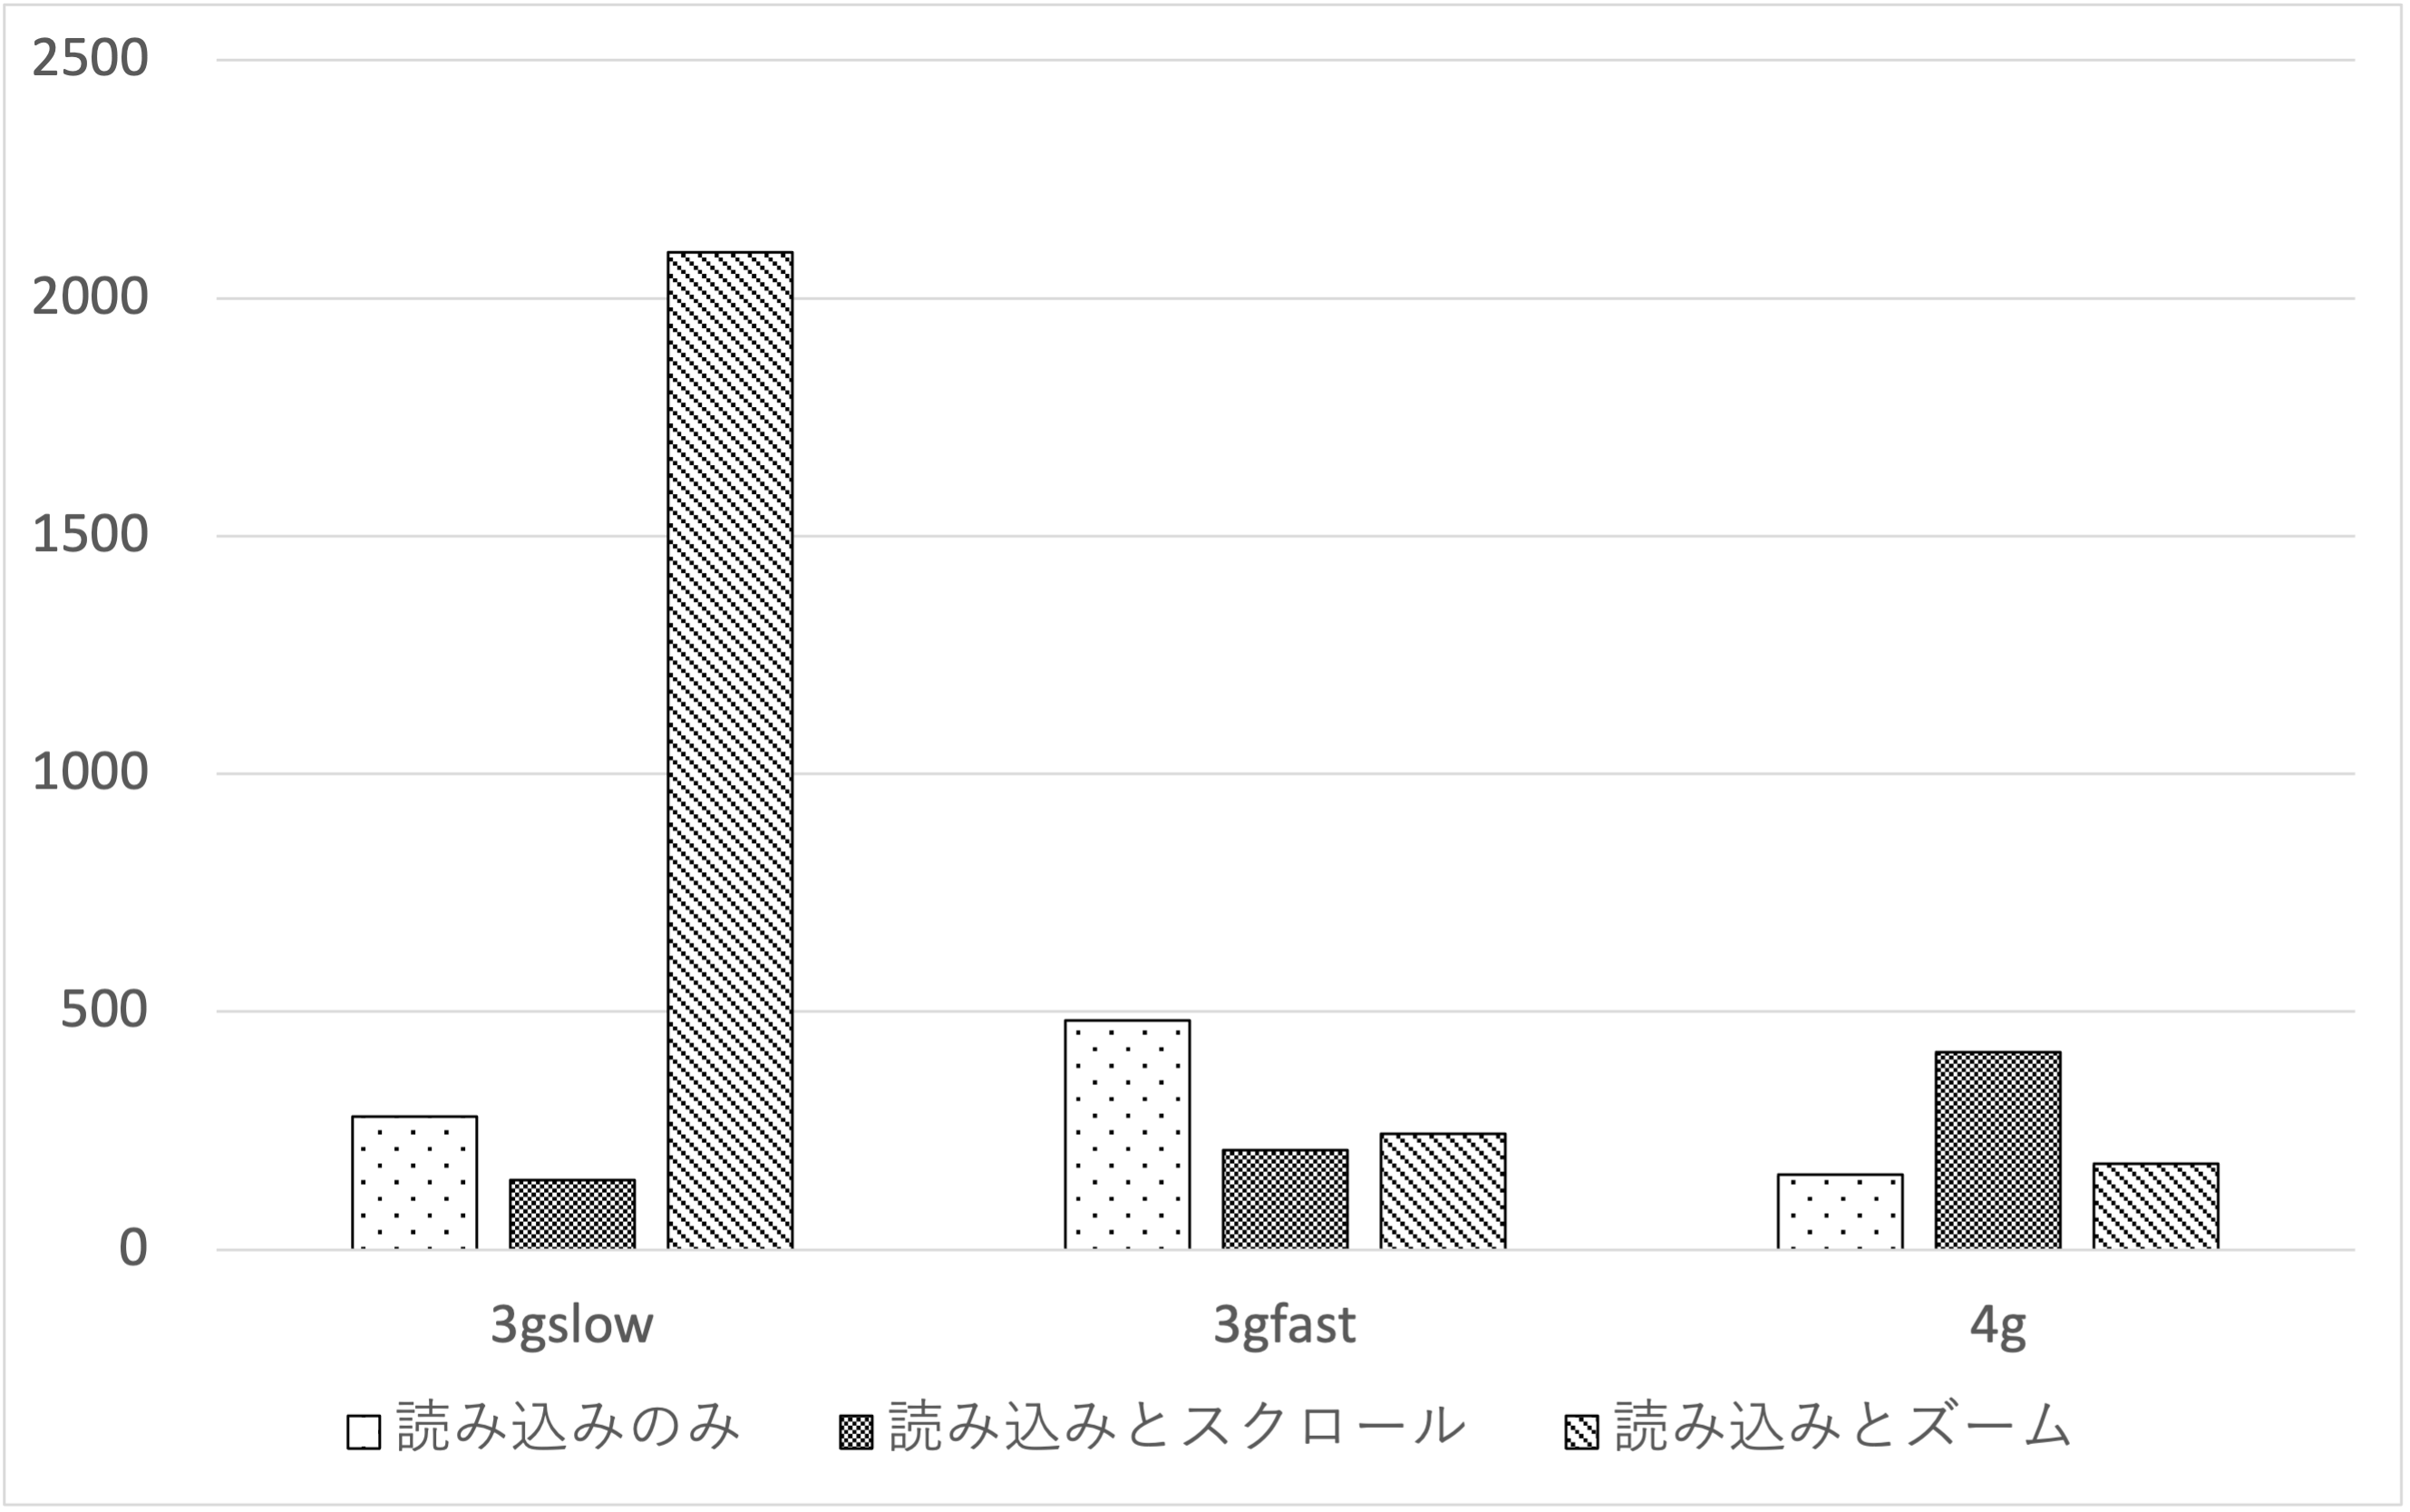
\includegraphics[width=\textwidth]{paper/images/sum_of_image_durations_with_service_worker.png}
  \caption{Service Workerを使用する場合の1都道府県当たりの画像の読み込み時間の合計平均[ミリ秒]}\label{figure:Service Workerを使用する場合の1都道府県当たりの画像の読み込み時間の合計平均}
\end{figure}

まずは、Service Workerを無効にした際のデータに着目する。ズーム倍率を1だけ増加させた場合は、読み込みのみの操作を行った場合と比べてほぼ2倍の画像の読み込み時間がかかっている。これは、ズーム倍率を1だけ増加させると、読み込む画像の枚数が2倍になるためである。しかし、1ページ下にスクロールした場合は、飲み込みのみの操作を行った場合と比べて読み込む画像の枚数が2倍に近いにもかかわらず画像の読み込み時間の増加率が低い。

次に、Service Workerを有効にした際のデータに着目すると、Service Workerを無効にした際のデータに比べて画像の読み込み時間が短いことが分かる。3gslowプロファイルを使用してズーム倍率を1だけ増加させた場合の画像の読み込み時間が比較的長いが、これは、一部の画像がService Workerによって正しくキャッシュされなかったことが原因である可能性がある。